\documentclass[a4paper, 12pt]{article}
    
\usepackage[left=3cm,right=3cm,top=1cm,bottom=2cm]{geometry}
\usepackage{amsmath,amsthm}
\usepackage{amssymb}
\usepackage{lipsum}
\usepackage[T1, T2A]{fontenc}
\usepackage[utf8]{inputenc}
\usepackage[bulgarian]{babel}
\usepackage[normalem]{ulem}
\usepackage{titlesec}
\usepackage{listingsutf8}
\usepackage{color}
\usepackage{graphicx}
\newcommand{\univname}{Софиийски университет "Св. Климент Охридски"\\Факултет по математика и информатика}

\definecolor{mygreen}{RGB}{28,172,0}
\definecolor{mylilas}{RGB}{170,55,241}

\lstset{language=Matlab,
    breaklines=true,
    morekeywords={matlab2tikz},
    keywordstyle=\color{blue},
    morekeywords=[2]{1}, keywordstyle=[2]{\color{black}},
    identifierstyle=\color{black},
    stringstyle=\color{mylilas},
    commentstyle=\color{mygreen},
    showstringspaces=false,
    numbers=left,
    numberstyle={\tiny \color{black}},
    numbersep=9pt
}

\setlength{\parindent}{0mm}

\begin{document}
\begin{titlepage}
\begin{center}
    
\vspace*{.06\textheight}
{\scshape\large \univname\par}\vspace{1.5cm}

{\huge \bfseries{Проект}\par}\vspace{0.7cm}
\textsc{\small по}\\[0.6cm]
\textsc{\Large Дифиренциални уравнения и приложения}\\[0.5cm]
\textsc{\normalsize спец. Информатика, 2 курс, зимен семестър,}\\[0.5cm]
\textsc{\normalsize учебна година 2017/18}\\[0.6cm]
\textsc{\large Тема И17-3}\\[3cm]
     
\begin{minipage}[t]{0.4\textwidth}
\begin{flushleft} \large
{\large \today}\\[1cm]
София
\end{flushleft}
\end{minipage}
\begin{minipage}[t]{0.4\textwidth}
\begin{flushright} \large
\emph{Изготвил:}\\[0.5cm]
Иво Алексеев Стратев\\[0.5cm]
Фак. номер: 45342\\[0.2cm]
Група: 3\\[2cm]
Оценка: .............................
\end{flushright}
\end{minipage}
\end{center}
\end{titlepage}

\tableofcontents

\listoffigures

\pagebreak

\section{Тема (Задание) на проекта}

\textbf{\textit{Задача 1.}} Дадена е задачата на Коши
\begin{align*} 
    xy' = 5y + 3x, \quad y(2) = 1
\end{align*}


1. Напишете интегрално уравнение еквивалентно
на дадената задача и по метода на Пикар дефинирайте
редица от последователни приближения на решението
на тази задача.


2. Начертайте с различни цветове графиките на
първото, третото и петотоприближение в интервала $[1, \; 3]$.
С подходящ числен метод, вграден в Matlab, намерете
числено решение на дадената задача и начертайте с 
черен цвят неговата графика в същия интервал. \\


\textbf{\textit{Задача 2.}} Дадена е системата
\begin{align*} 
    \begin{array}{|l}
        \dot{x} = -2x + 4y \\
        \dot{y} = x(x + 4)    
    \end{array}
\end{align*}


1. Намерете нейните равновесни точки. Начертайте
векторно поле на тази система в правоъгълник, който
съдържа намерените равновесни точки и с негова
помощ изследвайте за устойчивост равновесните положения.


2. За решението на задачата на Коши за дадената система
с начални условия $x(0) = x_0, \; y(0) = y_0$ направете
анимация на движението на точката $(x(t), \; y(t))$
във фазовата равнина за $t \in [0, \; 8]$, като точката
$(x_0, \; y_0)$ се въвежда чрез кликване с мишката
в избрания правоъгълник.

\pagebreak

\section{Решение на Задача 1}

\subsection{Теоретична част}

При $x = 0$ получаваме $0 = 5y$ или $y = 0$,
тоест получаваме точката $(0, \; 0)$. \\


Нека $x \neq 0$ тогава можем да разделим на $x$
и така получаваме $y' = \frac{5}{x}y + 3$.
Ще сменим името на променливата от $x$ на $s$.
Тогава уравнението добива вида:
\begin{align*}
    \frac{\mathrm d}{\mathrm d s}y = \frac{5}{s}y + 3
\end{align*}

Интегрираме уравението от двете страни в граници от $2$ до $x$ и получаваме
\begin{align*}
    \displaystyle\int_2^x \frac{\mathrm d}{\mathrm d s}y(s) \; \mathrm d s = \displaystyle\int_2^x  \frac{5}{s}y(s) + 3 \; \mathrm d s \implies \\\\
    \displaystyle\int_2^x {\mathrm d y} = \displaystyle\int_2^x  \frac{5}{s}y(s) + 3 \; \mathrm d s \implies \\\\
    y(x) - y(2) = \displaystyle\int_2^x  \frac{5}{s}y(s) + 3 \; \mathrm d s \implies \\\\
    y(x) = y(2) + \displaystyle\int_2^x  \frac{5}{s}y(s) + 3 \; \mathrm d s \implies \\\\
    y(x) = 1 + \displaystyle\int_2^x  \frac{5}{s}y(s) + 3 \; \mathrm d s
\end{align*}

Полученото интегрално уравнение е еквивалентно
на дадената задача на Коши за $x \neq 0$. Така сведохме задачата на Коши
\begin{align*} 
    xy' = 5y + 3x, \quad y(2) = 1
\end{align*}

до следната еквивалентна на нея задача
\begin{align*} 
    y(x) = 1 + \displaystyle\int_2^x  \frac{5}{s}y(s) + 3 \; \mathrm d s, \quad y(0) = 0.
\end{align*}

Тоест от дифиренциално уравнение преминахме към интегрално. \\\\

Дефинираме следата редица от последователни приближения
на решението на тази задача по метода на Пикар
\begin{align*}
    y_0(x) \equiv y(2) = 1 \\\\
    \forall n \in \mathbb{N} \quad y_{n + 1}(x) = 1 + \displaystyle\int_2^x  \frac{5}{s}y_n(s) + 3 \; \mathrm d s
\end{align*}

\subsubsection{Символно решение на дадената задача на Коши}

Първо ще намерим общия вид на решенията на даденото
диференциялно уравнение. Както вече установихме при
$x = 0$ получаваме точката $(0, \; 0)$. При $x \neq 0$
получихме уравнението $y' = \frac{5}{x}y + 3$, което е
линейно диференциално уравнение и неговото общо решение е:
\begin{align*}
    y = e^{\int \frac{5}{x} \; {\mathrm d x}}\left(C + \int 3 e^{-\int \frac{5}{x} \; {\mathrm d x}} \; {\mathrm d x}\right)
\end{align*}

Използвайки факта, че ние търсим решение на дадената задача дефинирано в точката $2$,
получаваме
\begin{align*}
    y = x^5\left(C + 3\int x^{-5} \; {\mathrm d x}\right) \implies \\\\
    y = x^5(C - \frac{3}{4}x^{-4}) = Cx^5 - \frac{3}{4}x
\end{align*}

Използвайки началното условие намираме стойността на константа $C$
\begin{align*}
    y(2) = C.2^5 - \frac{3}{4}2 = C.2^5 - \frac{3}{2} = 1 \implies C = \frac{5}{2^6}
\end{align*}

Намерихме аналитично решение да дадената задача на Коши в квадратури
\begin{align*}
    y = \frac{5}{2^6}x^5 - \frac{3}{4}x
\end{align*}

\subsection{Матлаб код}

\lstinputlisting{tema3_zad1.m}

\subsubsection{Коментар към използваните вградени в Matlab функции}

За численето решение на задачата и за пресмятането на интегралите
от последователните приближение са използвани вградени в Matlab функции:
\textbf{\textit{ode45}} и \textbf{\textit{cumtrapz}}, които числено пресмятат
подадените им дифиренциално уравнение и определен интеграл започвайки
от точката на началното условие. Понеже тази точка за дадената задача
е $2$, която е средата на дадения интервал $[1, \; 3]$ то,
това налага последователно да се пресметнат числено
решенията в интервалите $[1, \; 2]$ и $[2, \; 3]$
и след това двете решения да бъдат долепени едно за друго. \\

Аналогично от математическа гледна точка графиката на решението в
интервала $[1, \; 3]$ също може да бъде разделена на две графики. Тоест
\begin{align*} 
    G(x, y)|_{x \in [1, \; 3]} = \{(x, \; y(x)) \; | \; x \in [1, \; 3]\} = \\
    = \{(x, \; y(x)) \; | \; x \in [1, \; 2]\} \cup \{(x, \; y(x)) \; | \; x \in [2, \; 3]\} = \\
    = G(x, y)|_{x \in [1, \; 2]} \cup G(x, y)|_{x \in [2, \; 3]}
\end{align*}

\subsection{Графики}

\begin{figure}[ht]
    \centering
    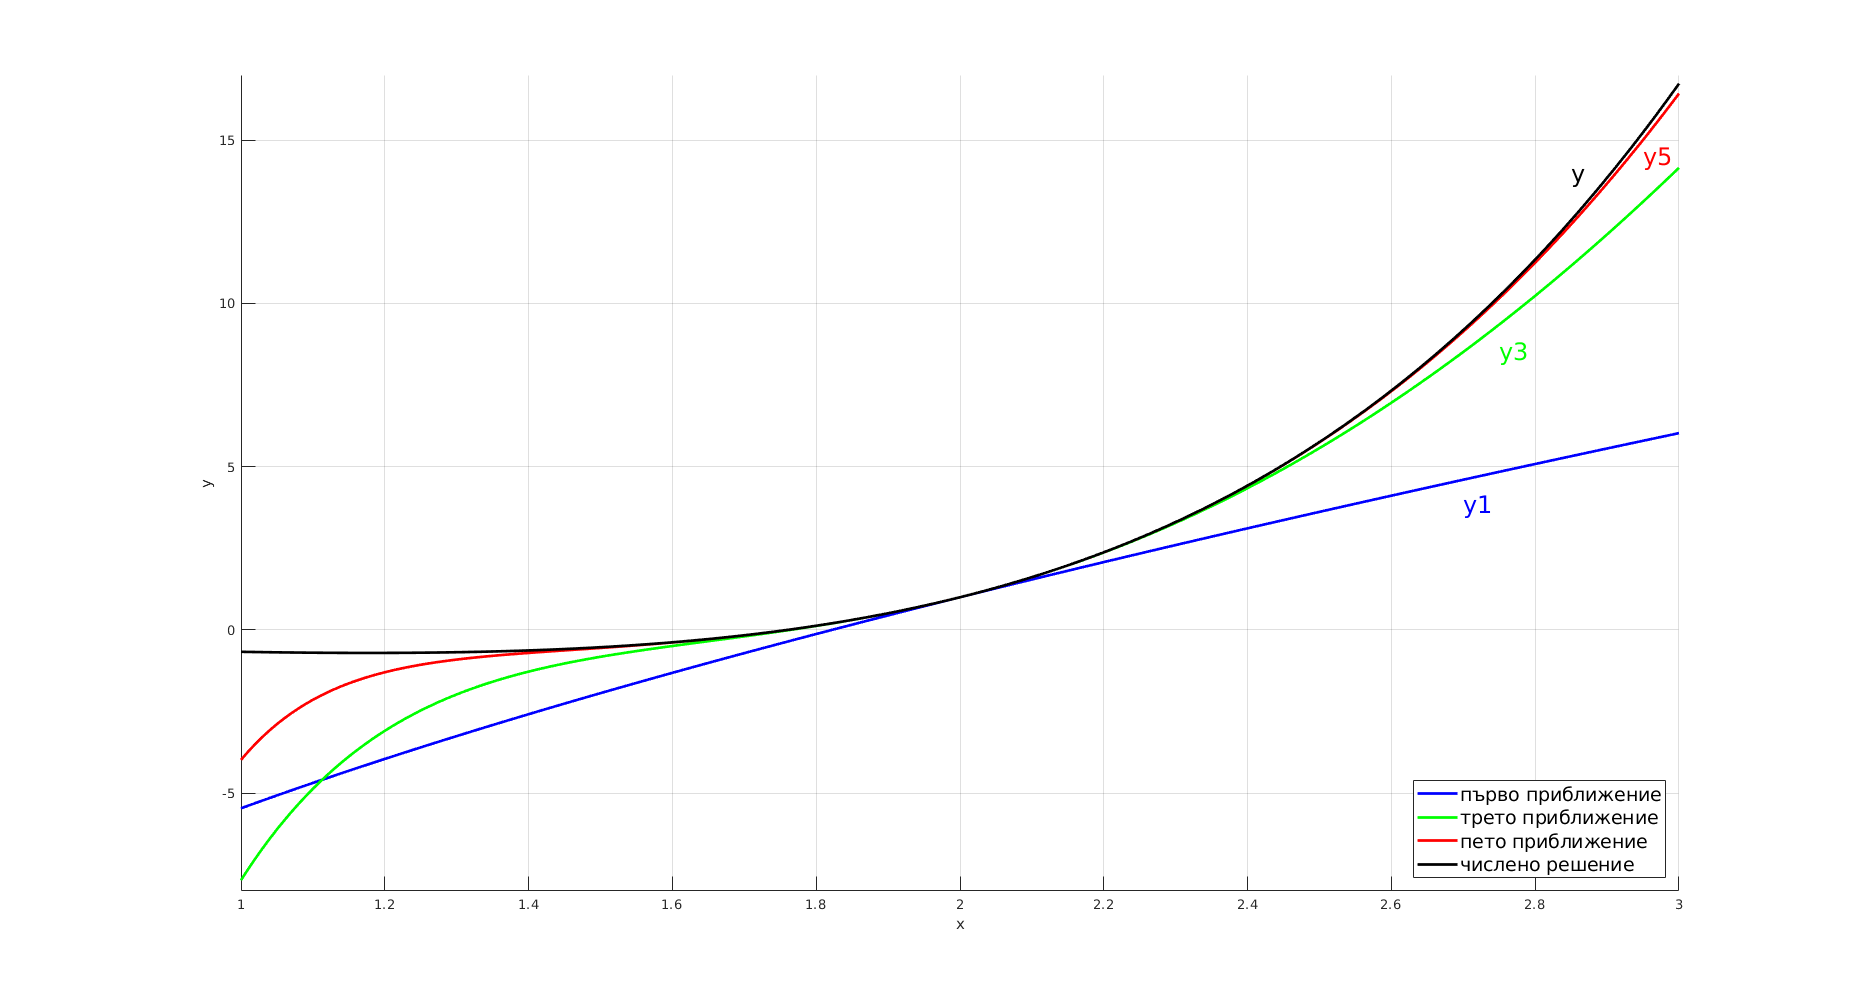
\includegraphics[width=\textwidth]{tema3_zad1.png}
    \caption{Графки на първото, третото и петото приближение по метода на Пикар и графика на численото решение в интервала $[1, \; 3]$}
\end{figure}

\subsection{Коментари към получените с Matlab резултати}

На графиката са начертани графиките на
първото приближение $y_1$ със син цвят,
третото приближение $y_3$ със зелен цвят
и с петото приближение $y_5$ с червен цвят,
получени по метода на Пикар в интервала $[1, \; 3]$.
С черен цвят е начертана графиката на полученото числено
решение на дадената задача на Коши също в интервала $[1, \; 3]$.

\section{Решение на Задача 2}

\subsection{Теоретична част}

Търсим равновесните точки на системата
\begin{align*} 
    \begin{array}{|l}
        \dot{x} = -2x + 4y \\
        \dot{y} = x(x + 4).    
    \end{array}
\end{align*}

Това са точките за нулевите вектори от векторното поле, породено от системата.

\begin{align*} 
    \begin{array}{|l}
        \dot{x} = 0 \\
        \dot{y} = 0
    \end{array} \implies \begin{array}{|l}
        -2x + 4y = 0 \\
        x(x + 4) = 0    
    \end{array} \implies \begin{array}{|l}
        y = \frac{x}{2} \\
        x(x + 4) = 0
    \end{array} \implies \{(0, \; 0), \; (-4, \; -2)\}
\end{align*}

С помощта на Matlab ще начертаем векторното
поле на дадената система и чрез него ще изследваме
за устойчивост намерените равновесни точки.

\subsection{Код на Matlab изчертващ векторното поле на системата}

\lstinputlisting{vectorField.m}

\subsection{Графика на изчертаното векторно поле на системата}

\begin{figure}[ht]
    \centering
    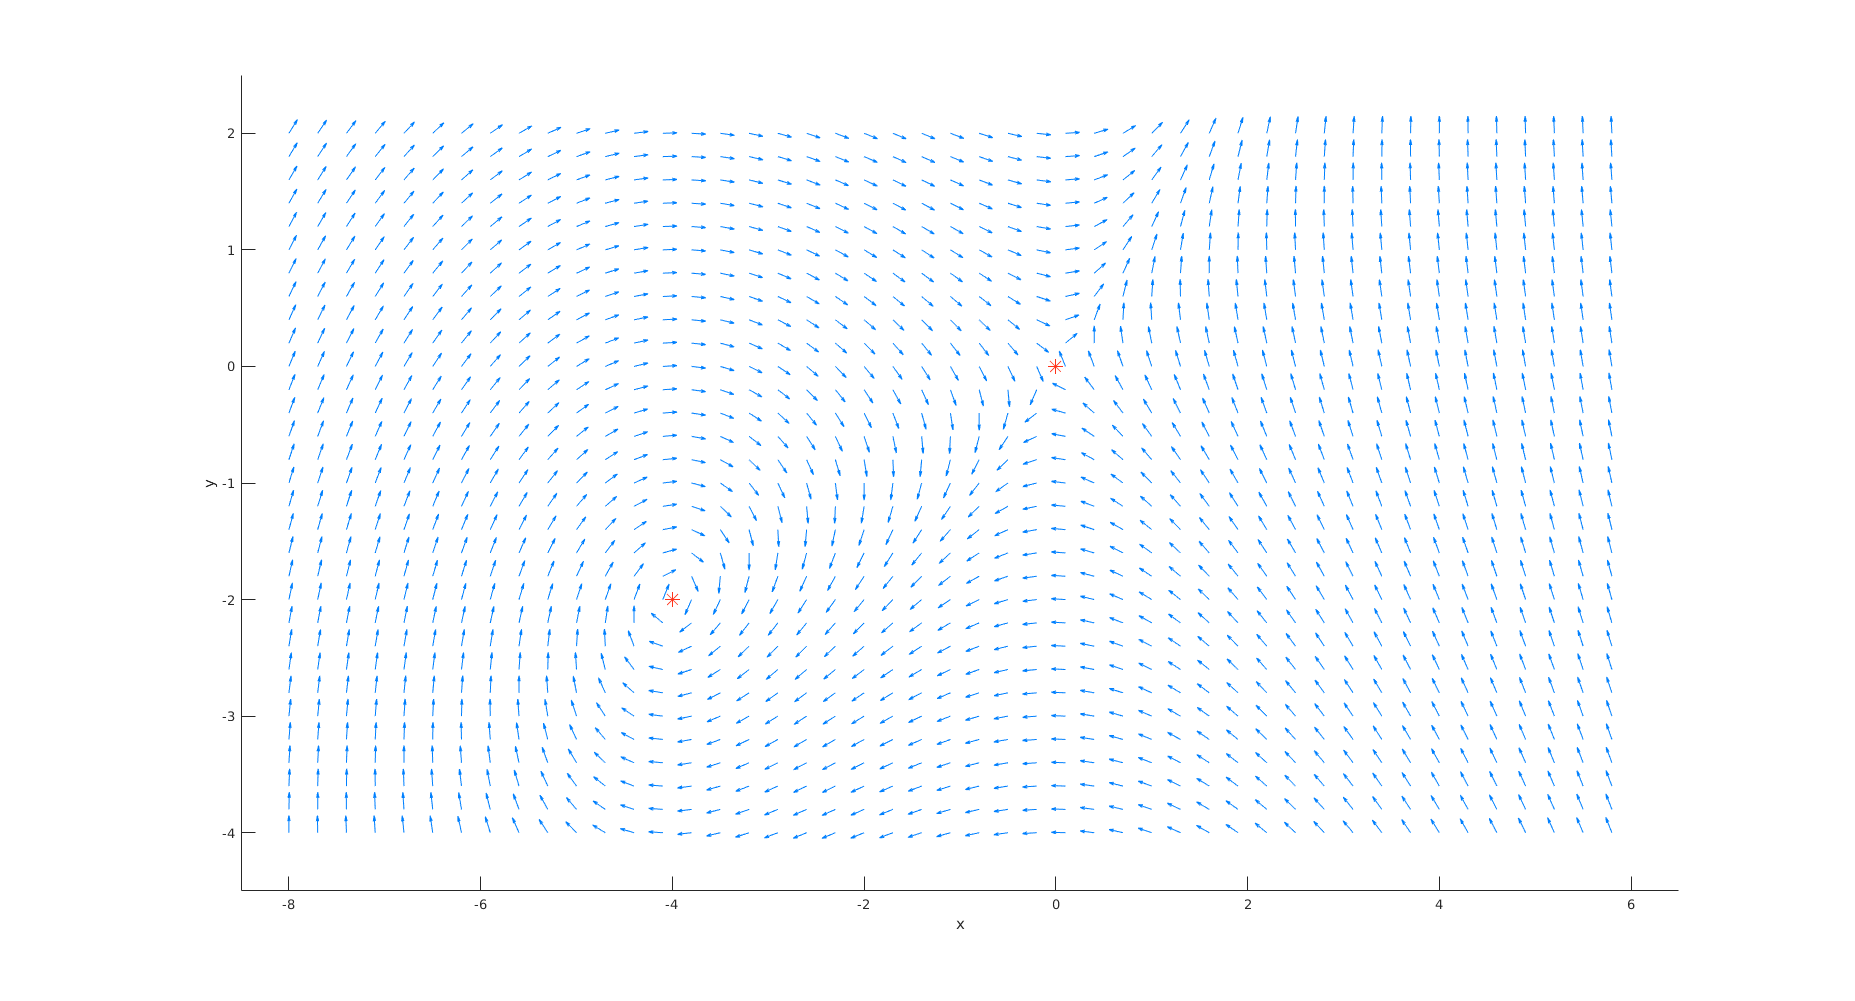
\includegraphics[width=\textwidth]{vectorField.png}
    \caption{Графкика на векторното поле на дадената система изчертано в подходящ правоъгълник съдържащ равновесните точки на системата}
\end{figure}

\subsection{Коментари към изчератаното с Matlab векторно поле}

Както лесно можем да забележим в околност на точката $(0, \; 0)$ фазовия
портрет на системата има вид на седло. Тоест точката $(0, \; 0)$ е неустойчива.
в околност на точката $(-4, \; -2)$ фазовия портрет системата има вид на
устойчив фокус и следователно точката $(-4, \; -2)$ е асимптотически устойчива.

\subsection{Матлаб код}

\lstinputlisting{tema3_zad2.m}

\subsection{Графики}

\begin{figure}[ht]
    \centering
    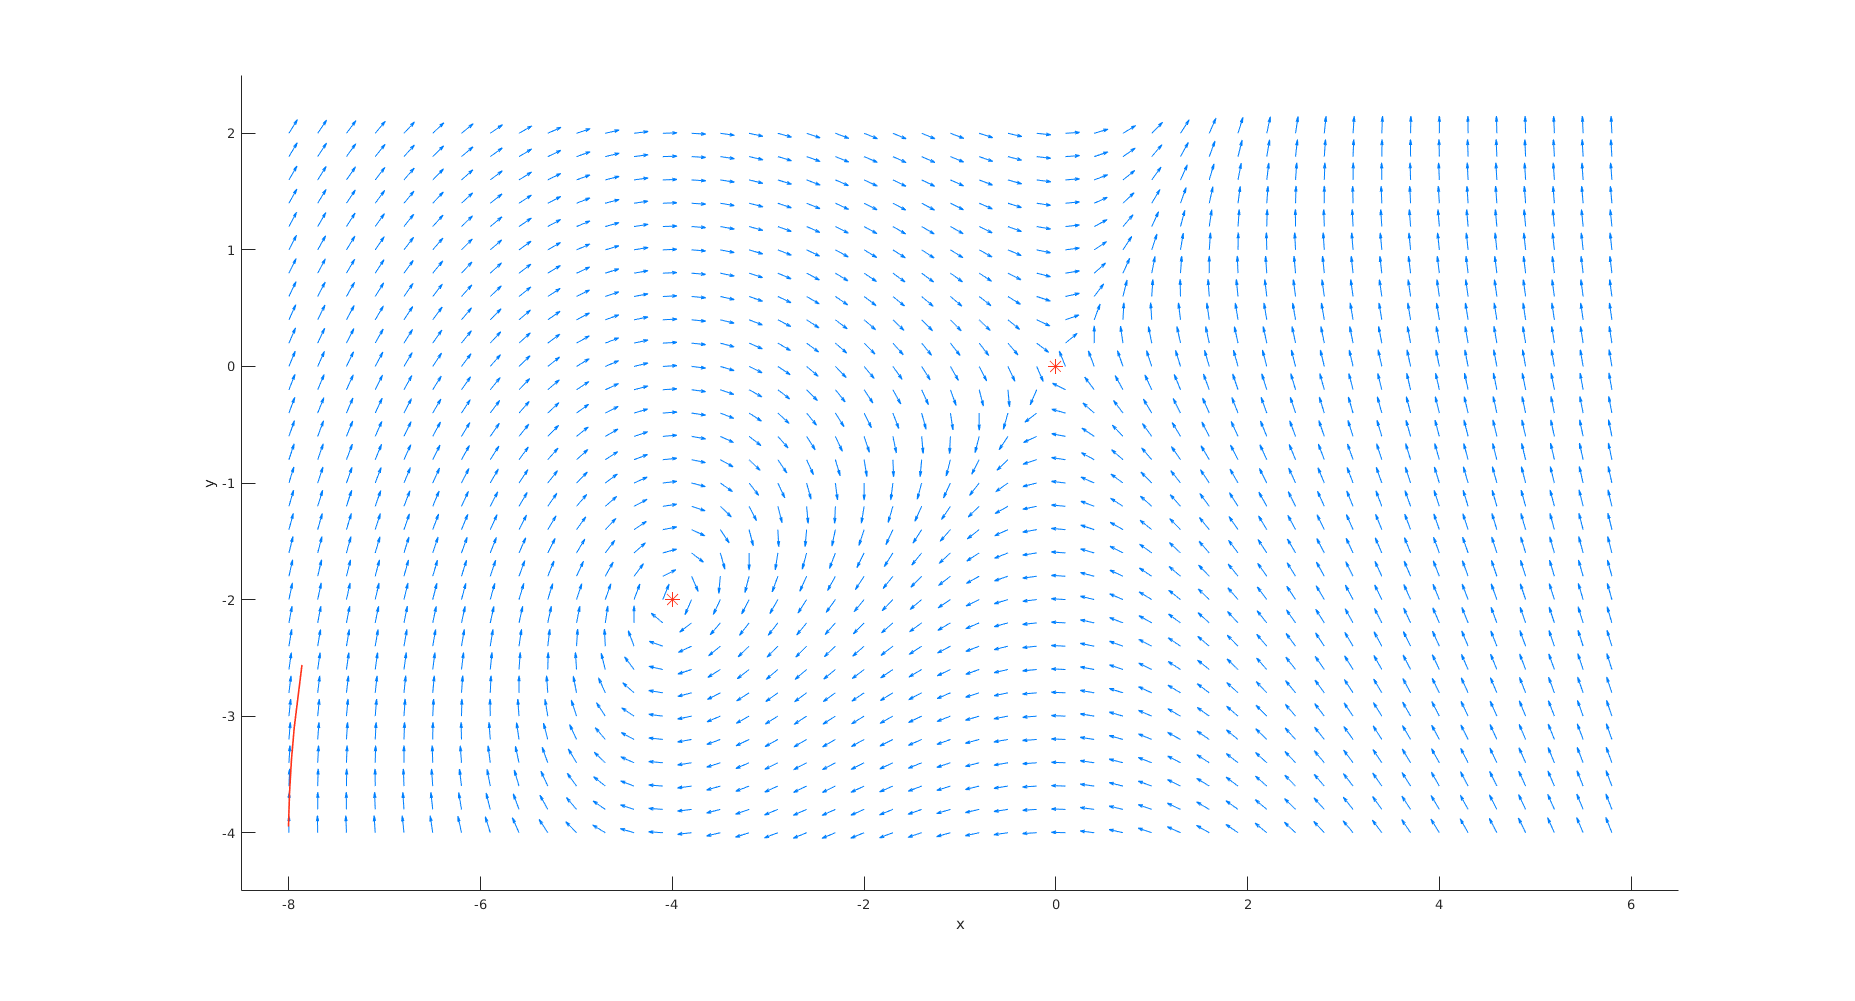
\includegraphics[width=\textwidth]{move1.png}
    \caption{Кадър 1 от анимация на движение на точка във фазовата равнина на системата}
\end{figure}

\begin{figure}[ht]
    \centering
    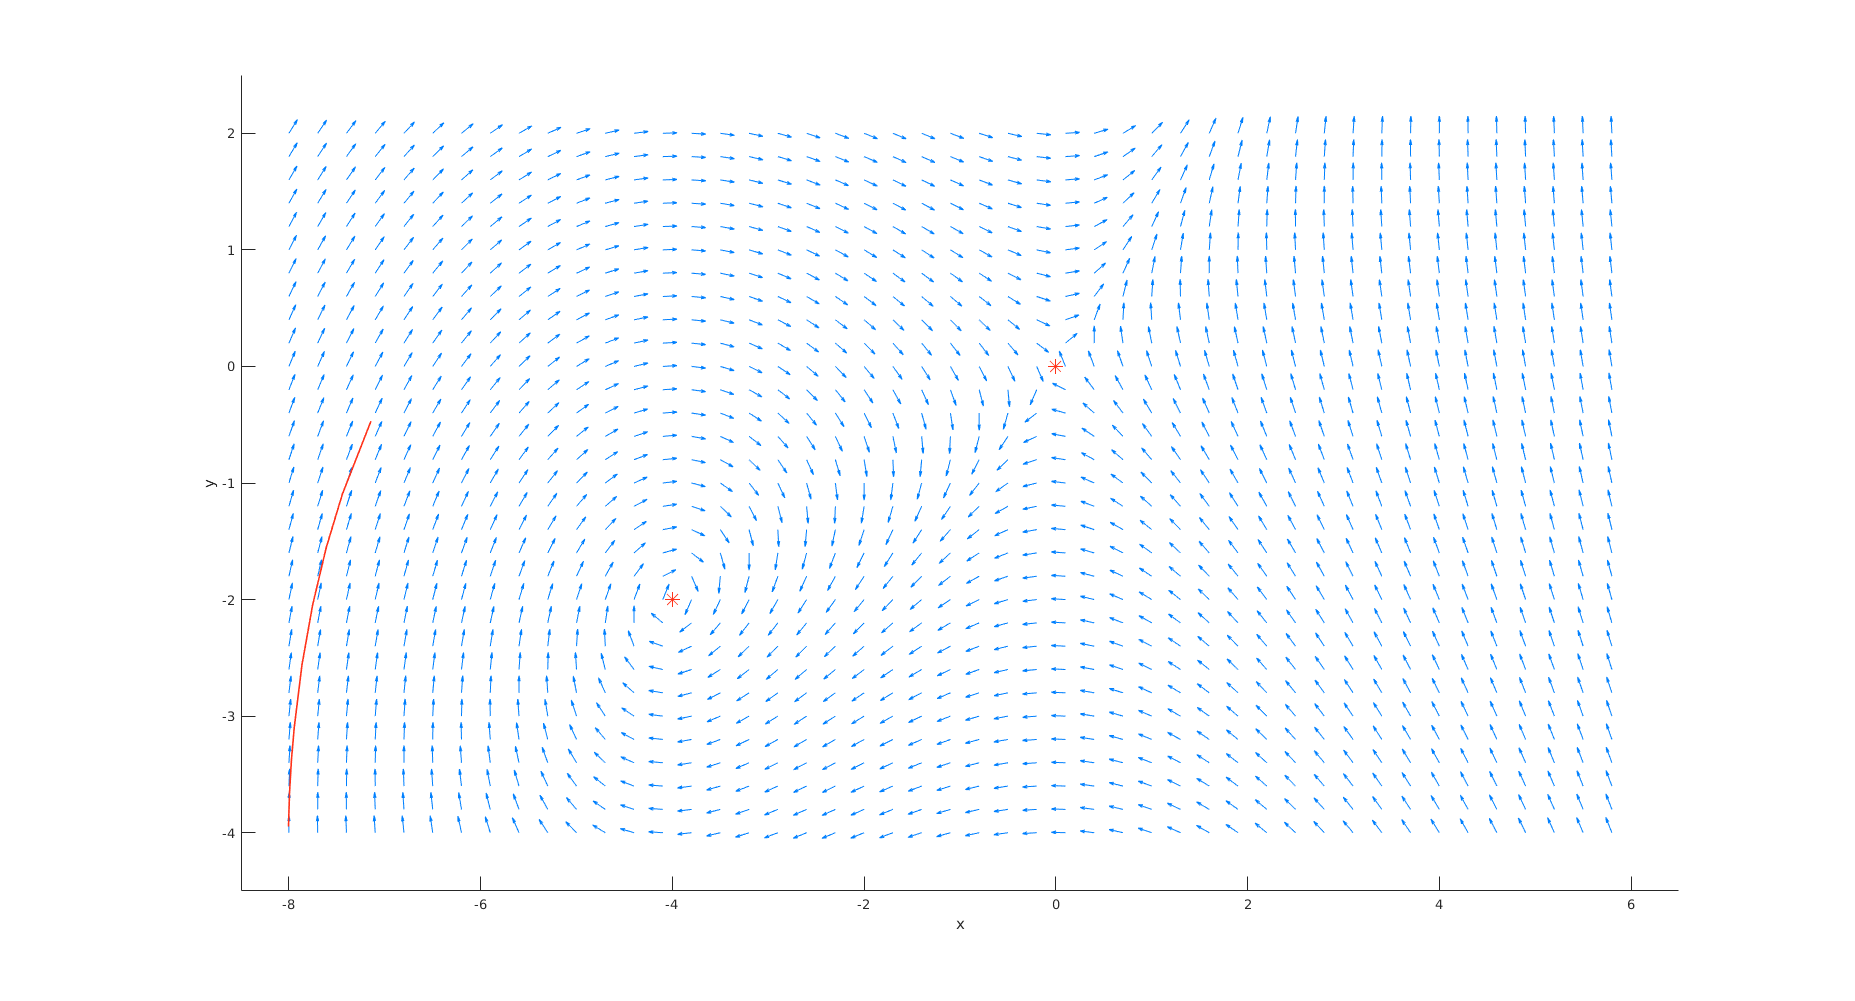
\includegraphics[width=\textwidth]{move2.png}
    \caption{Кадър 2 от анимация на движение на точка във фазовата равнина на системата}
\end{figure}

\begin{figure}[ht]
    \centering
    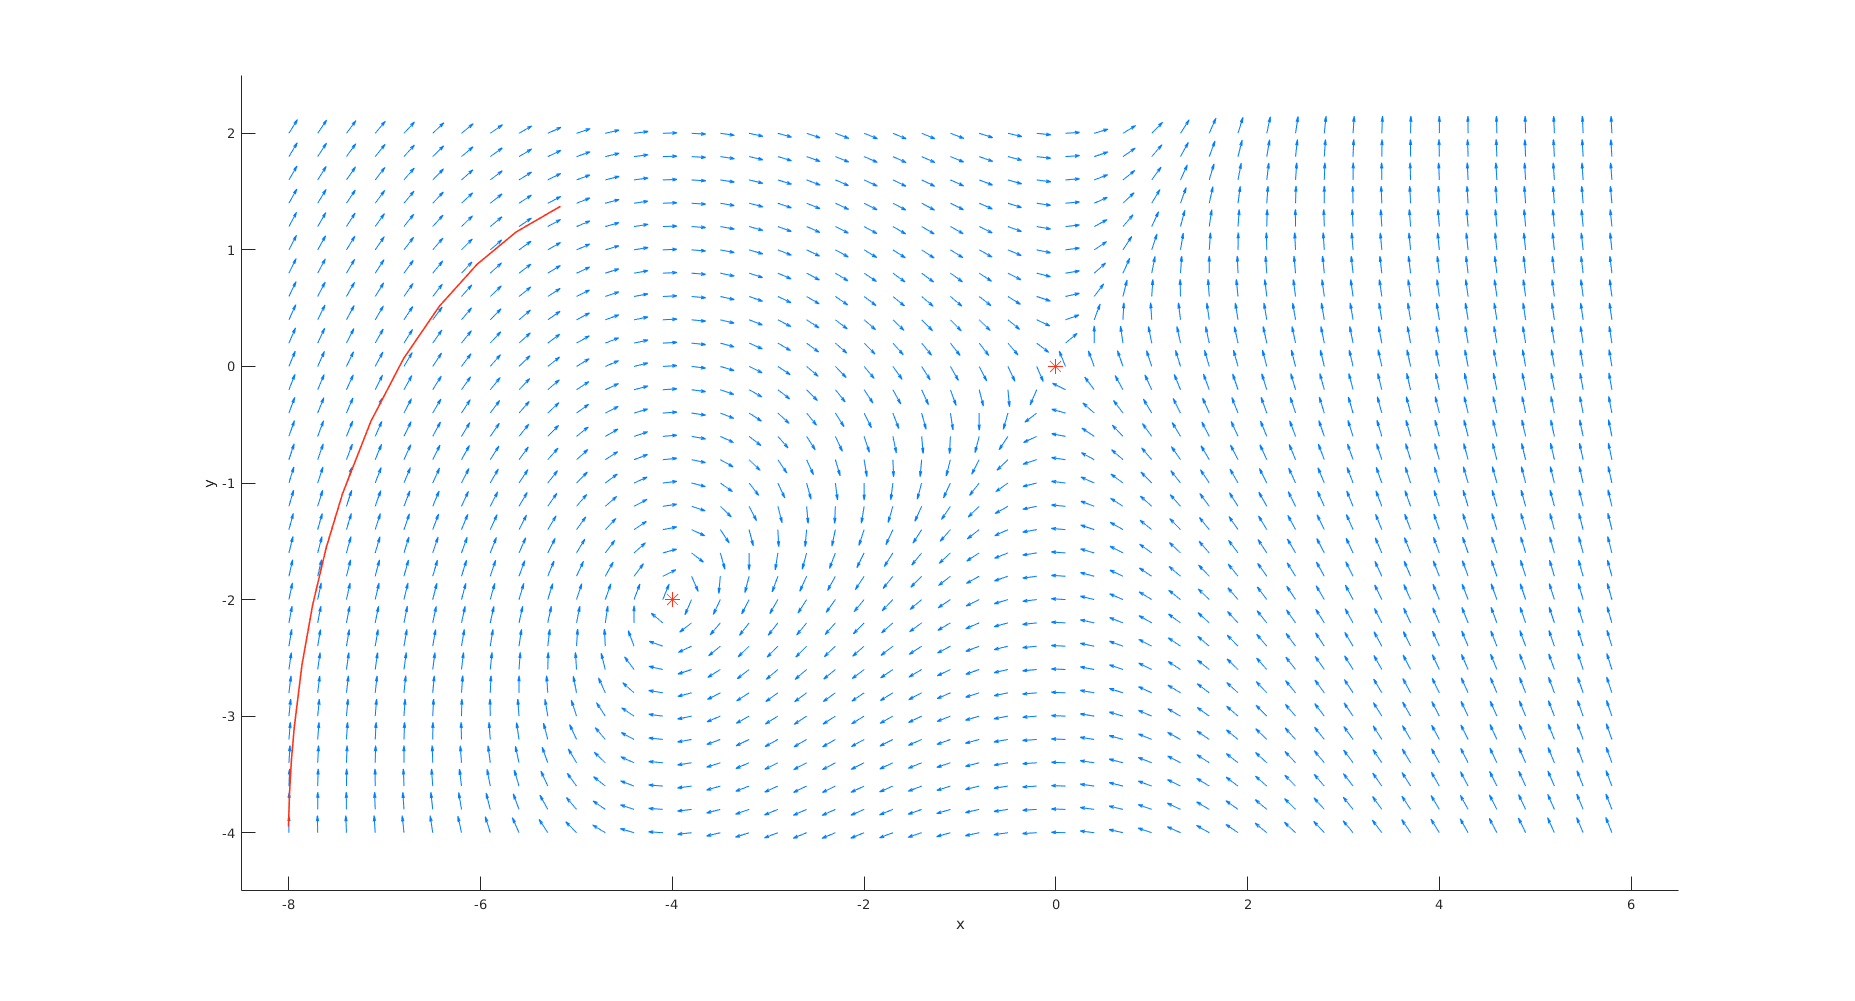
\includegraphics[width=\textwidth]{move3.png}
    \caption{Кадър 3 от анимация на движение на точка във фазовата равнина на системата}
\end{figure}

\begin{figure}[ht]
    \centering
    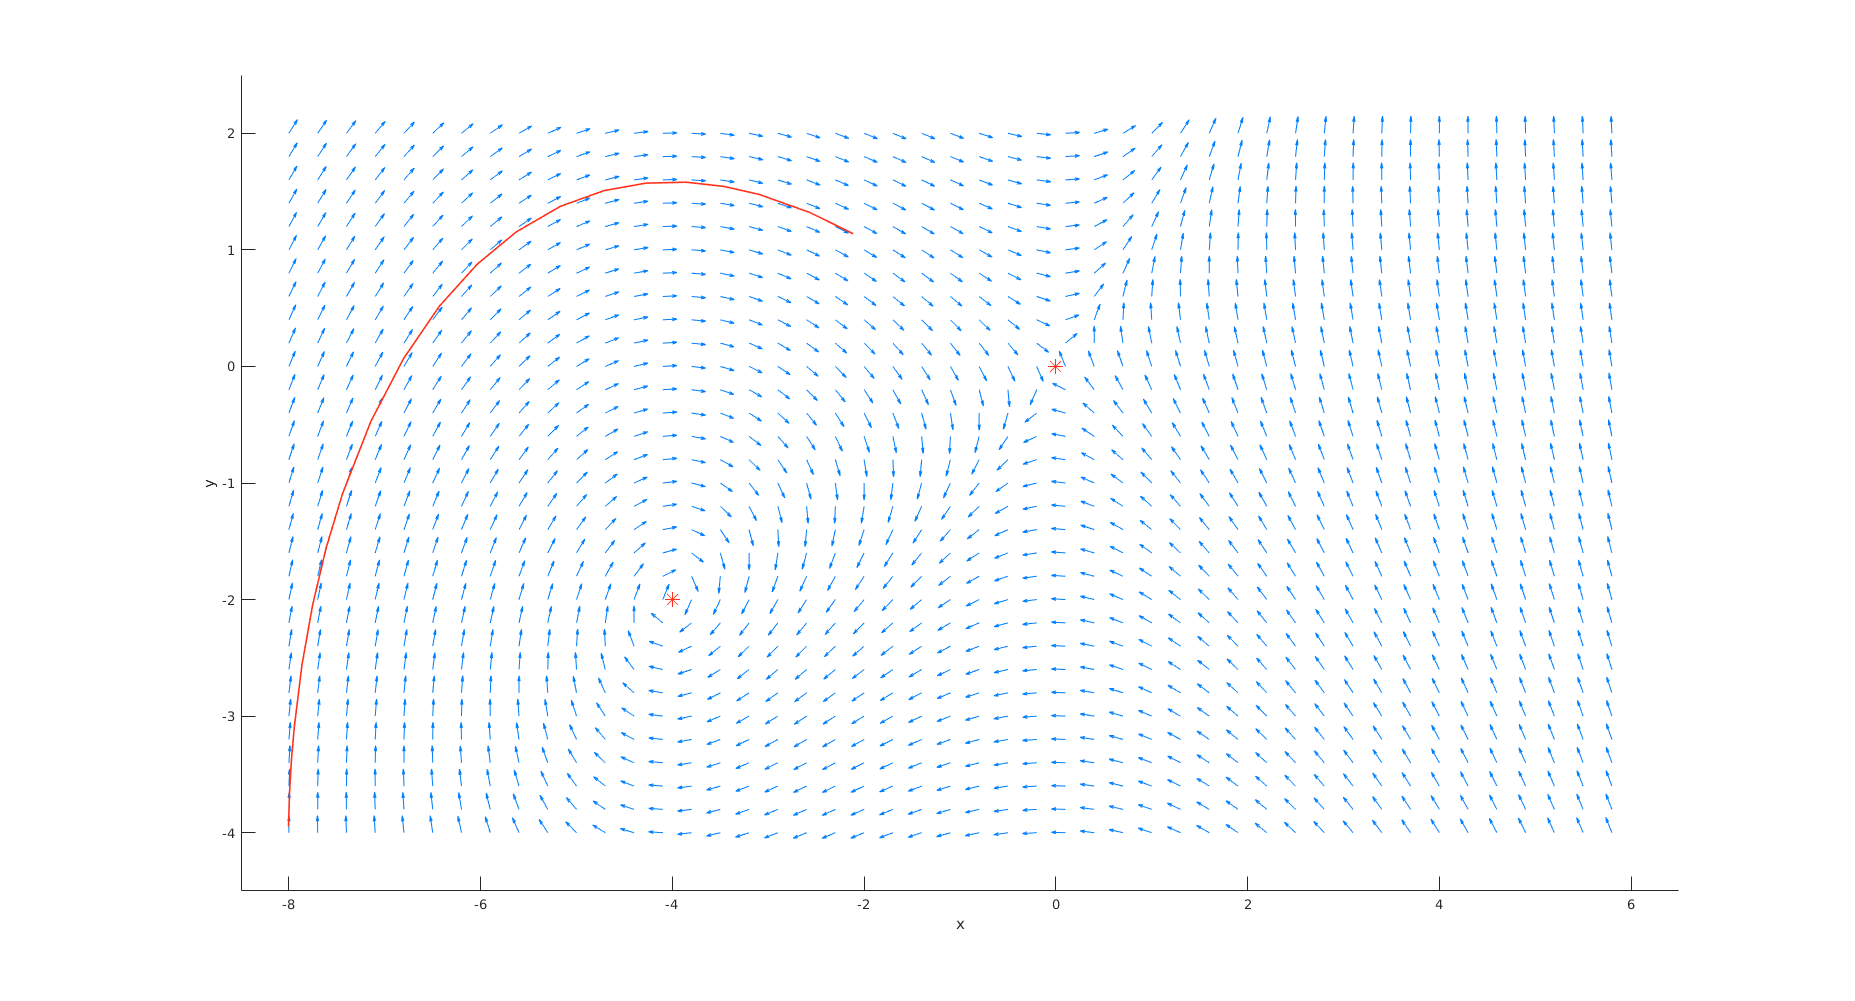
\includegraphics[width=\textwidth]{move4.png}
    \caption{Кадър 4 от анимация на движение на точка във фазовата равнина на системата}
\end{figure}

\begin{figure}[ht]
    \centering
    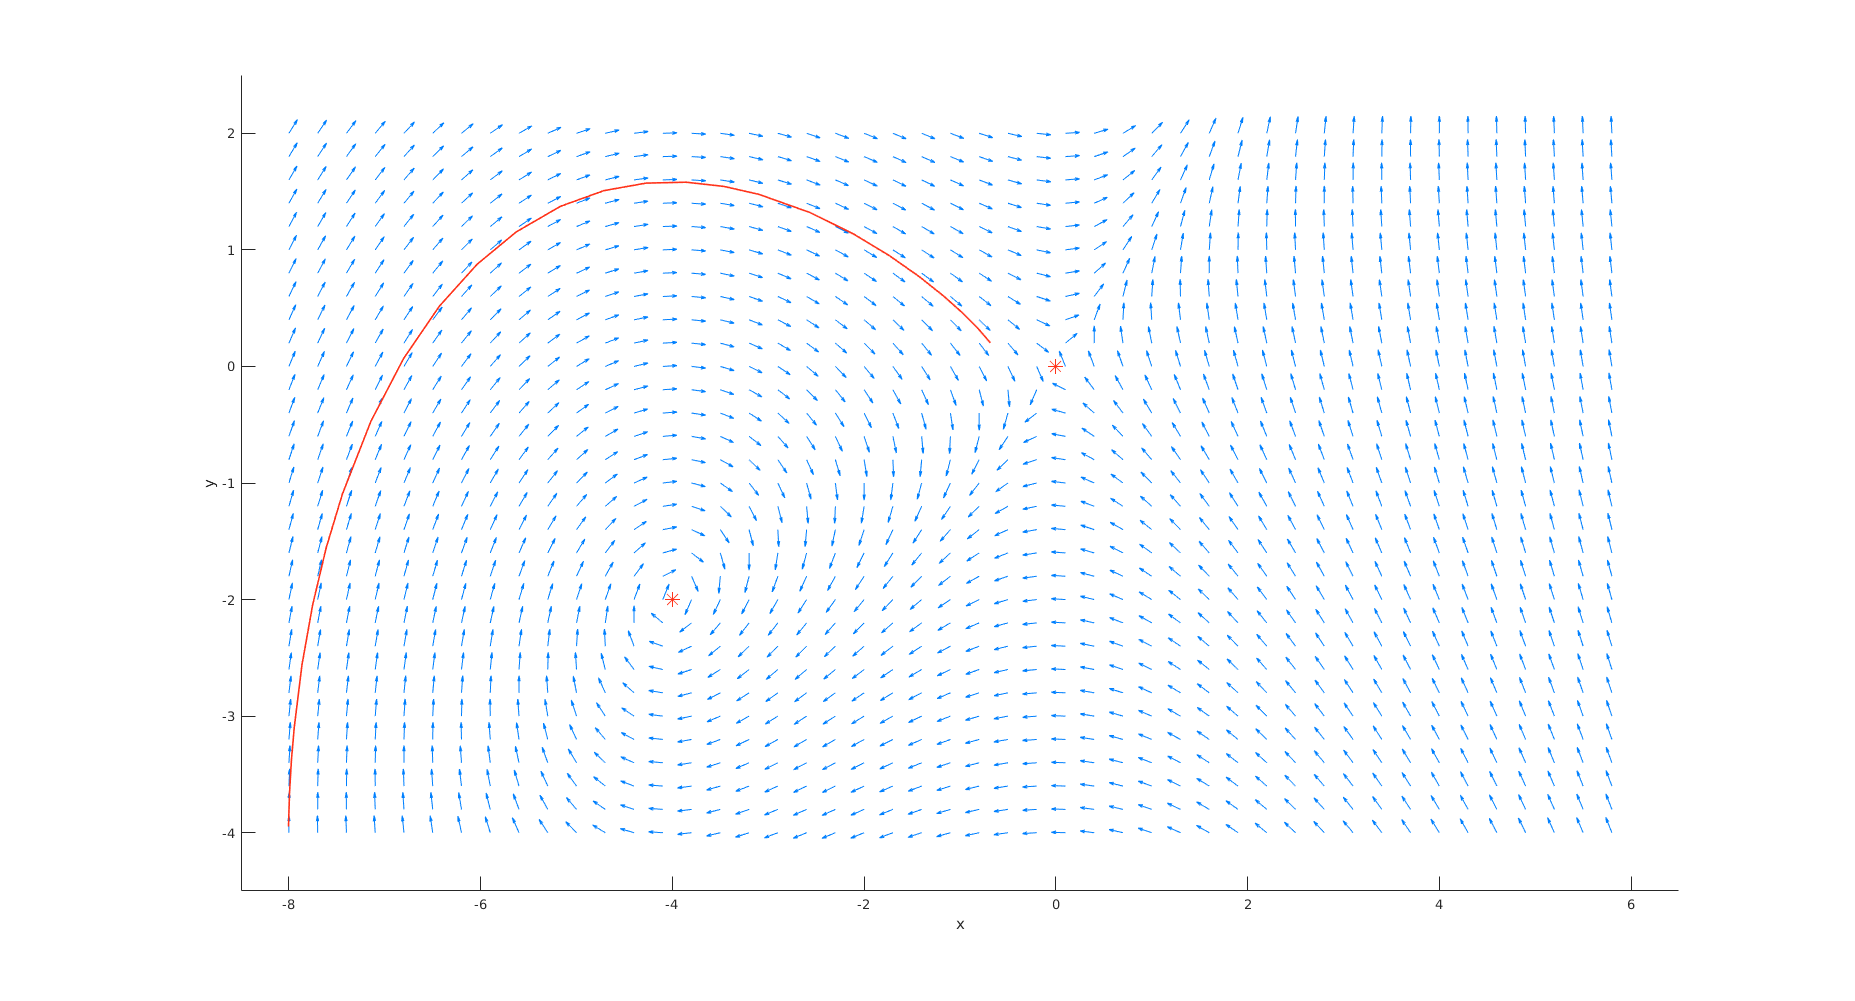
\includegraphics[width=\textwidth]{move5.png}
    \caption{Кадър 5 от анимация на движение на точка във фазовата равнина на системата}
\end{figure}

\begin{figure}[ht]
    \centering
    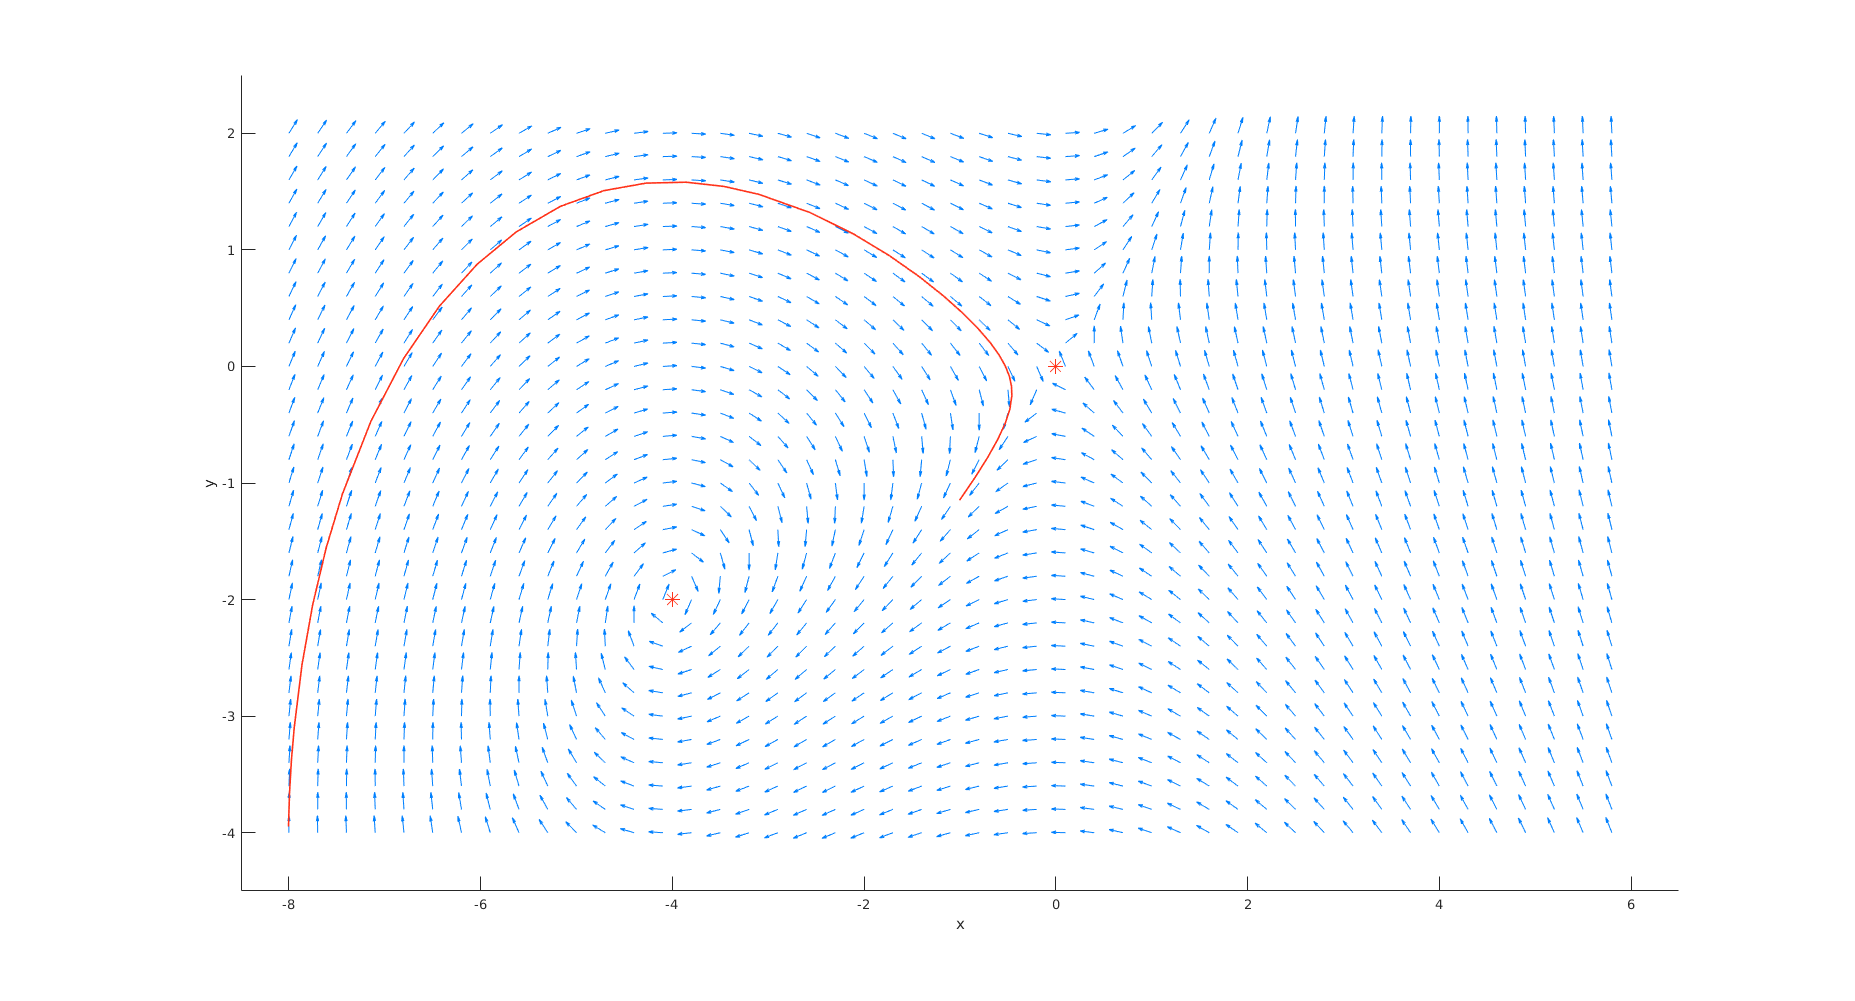
\includegraphics[width=\textwidth]{move6.png}
    \caption{Кадър 6 от анимация на движение на точка във фазовата равнина на системата}
\end{figure}

\begin{figure}[ht]
    \centering
    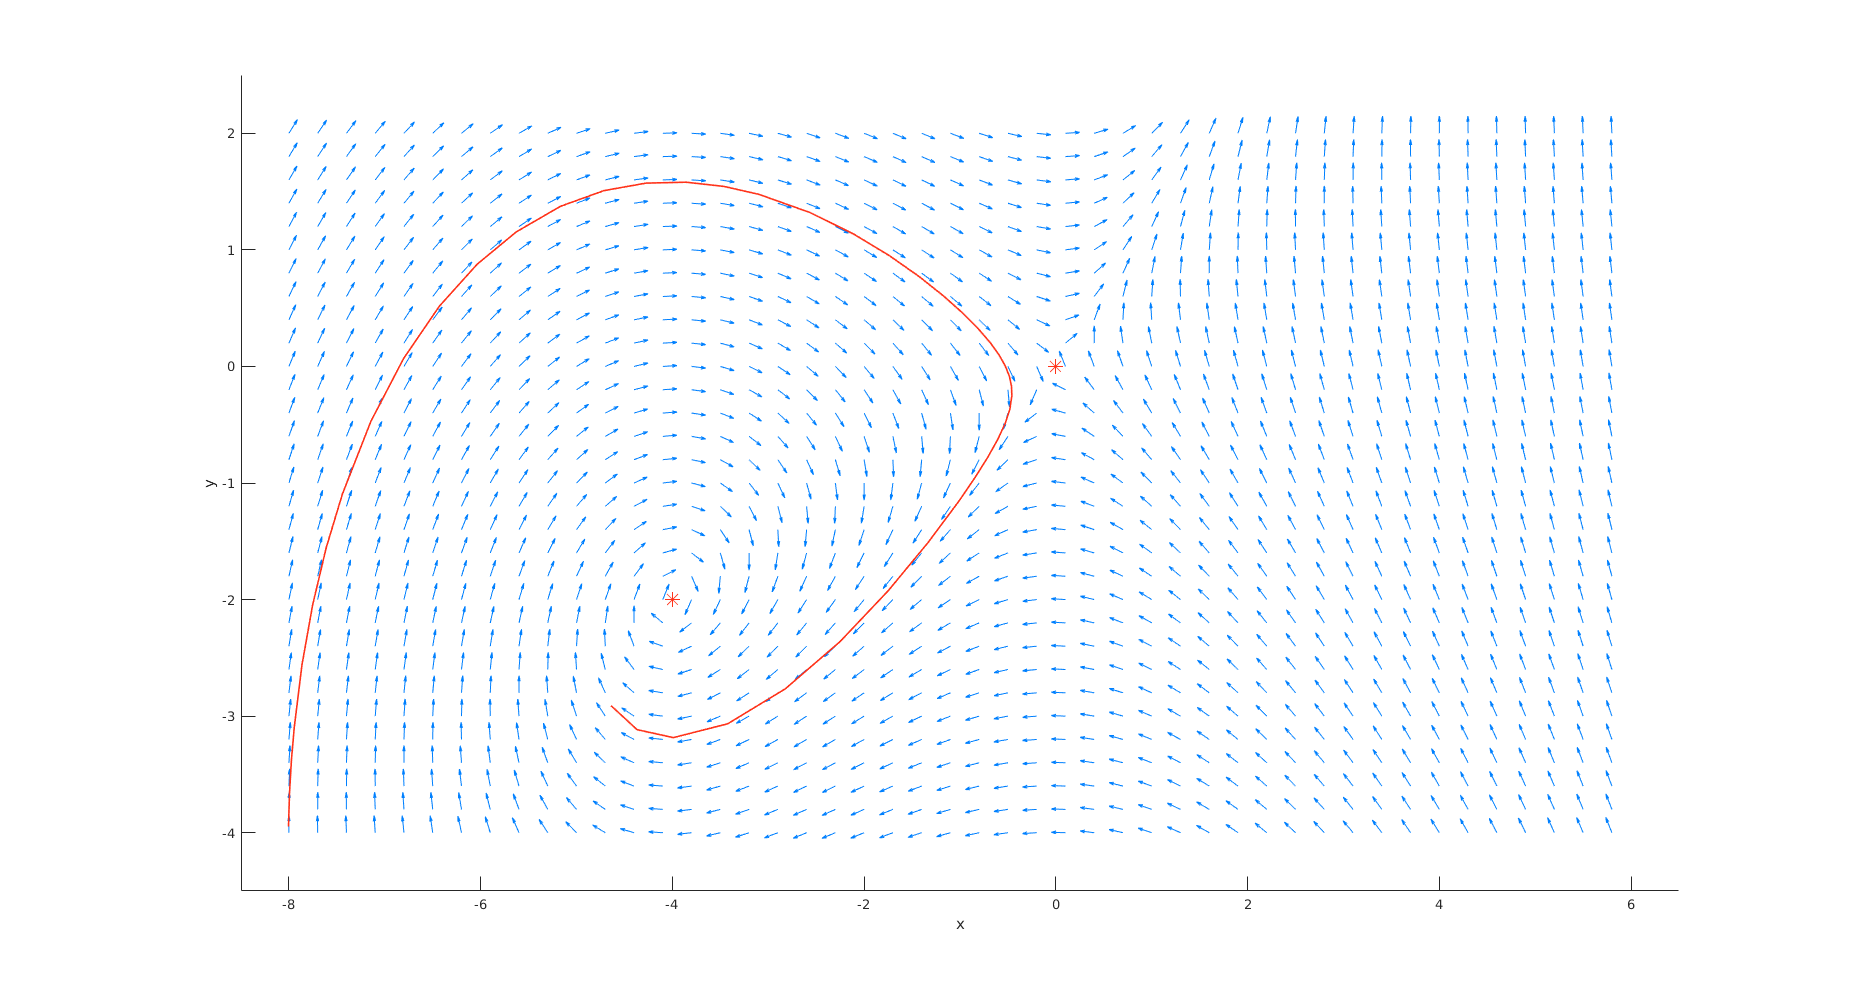
\includegraphics[width=\textwidth]{move7.png}
    \caption{Кадър 7 от анимация на движение на точка във фазовата равнина на системата}
\end{figure}

\begin{figure}[ht]
    \centering
    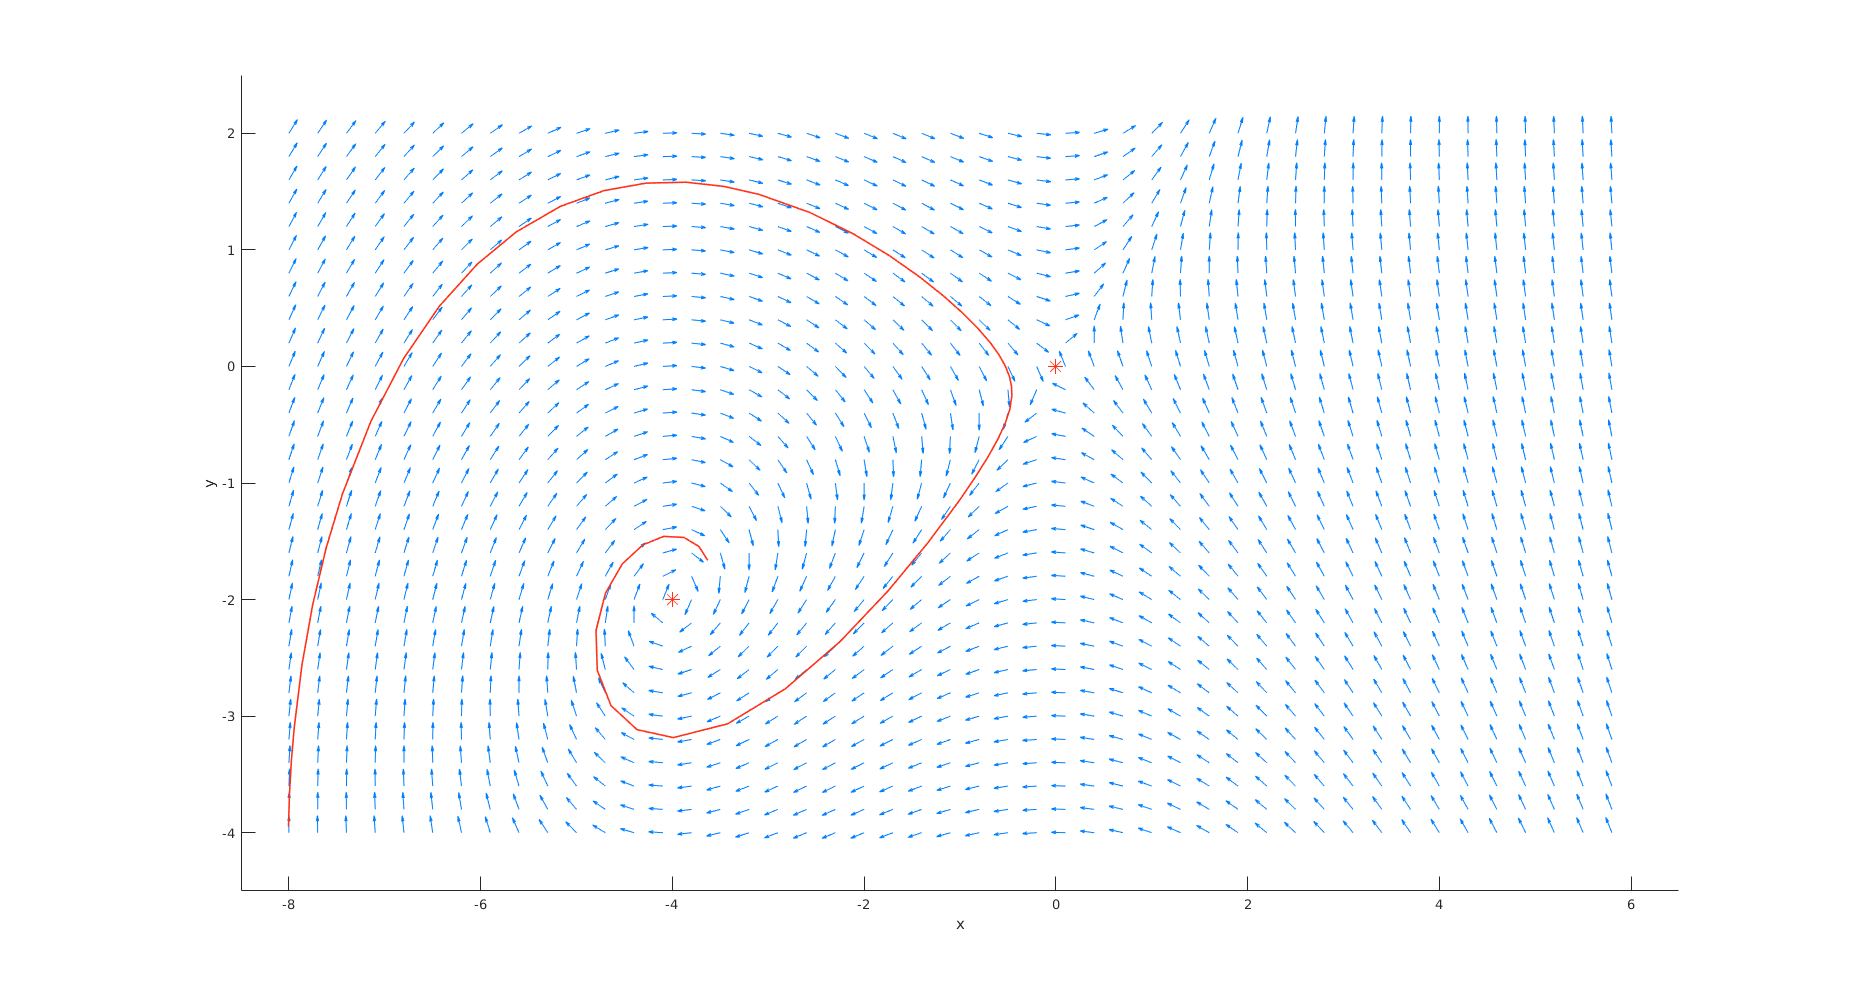
\includegraphics[width=\textwidth]{move8.png}
    \caption{Кадър 8 от анимация на движение на точка във фазовата равнина на системата}
\end{figure}

\begin{figure}[ht]
    \centering
    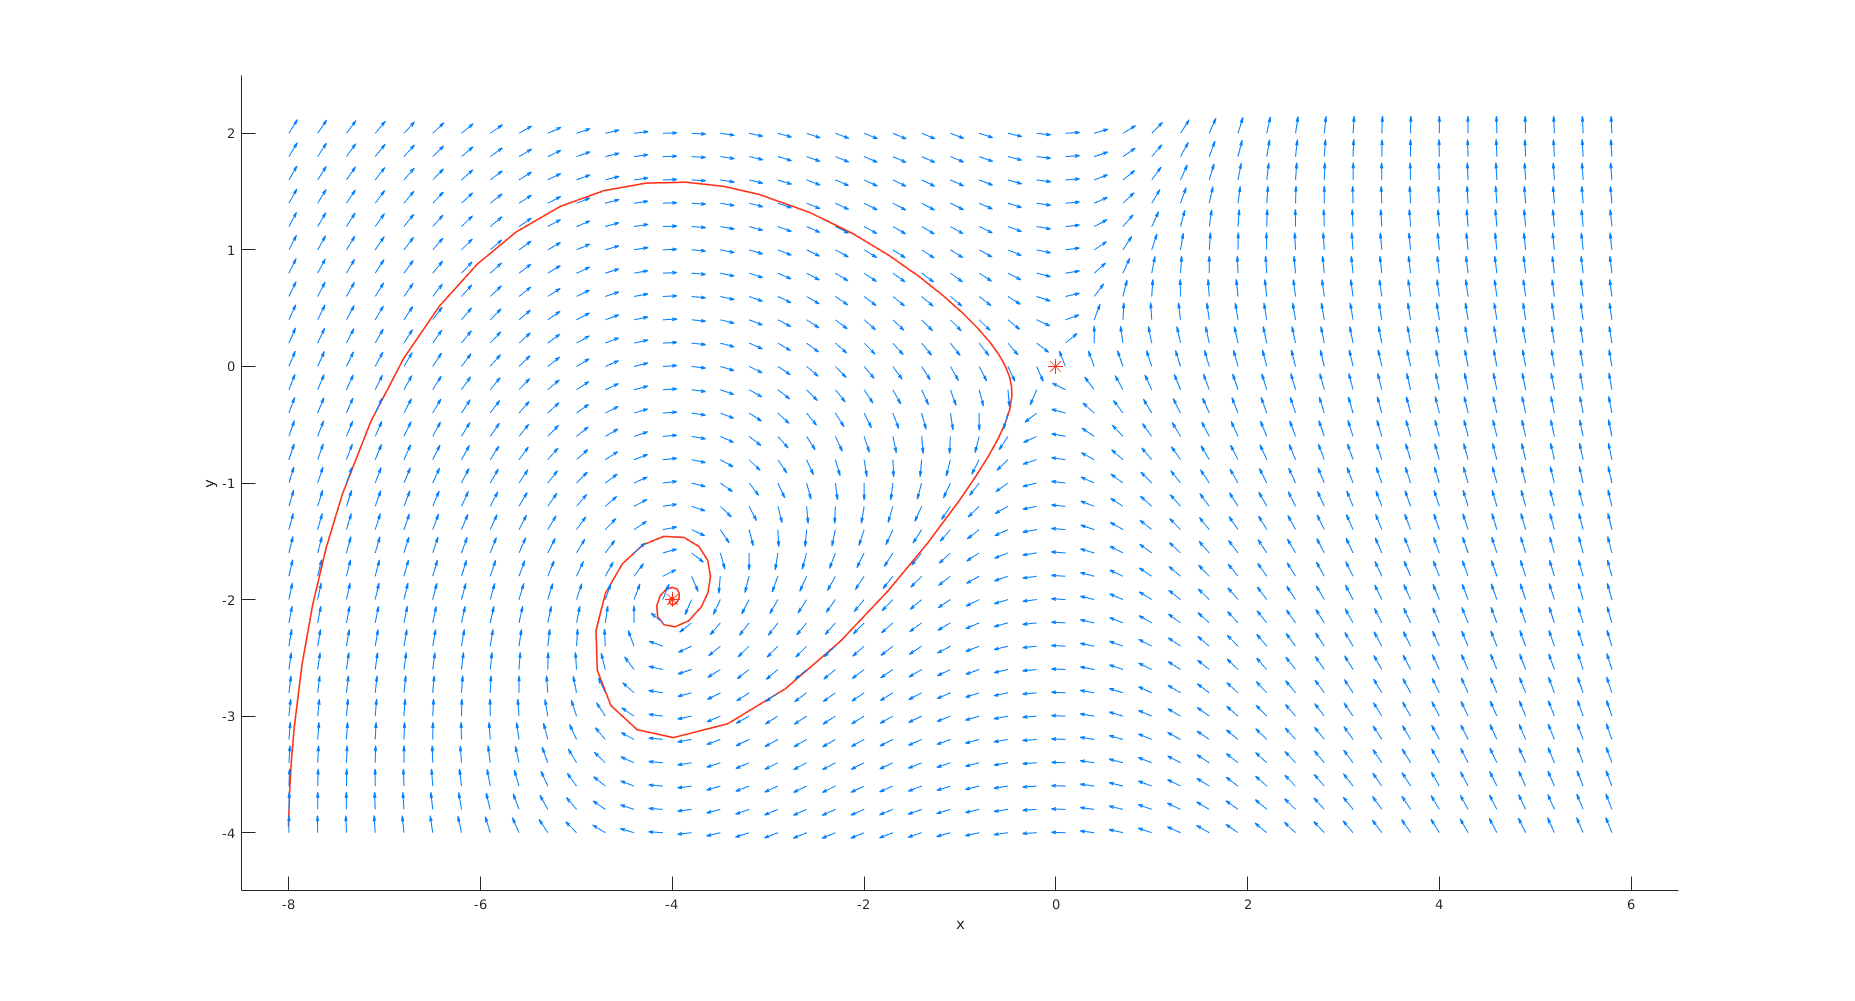
\includegraphics[width=\textwidth]{move9.png}
    \caption{Кадър 9 от анимация на движение на точка във фазовата равнина на системата}
\end{figure}

\begin{figure}[ht]
    \centering
    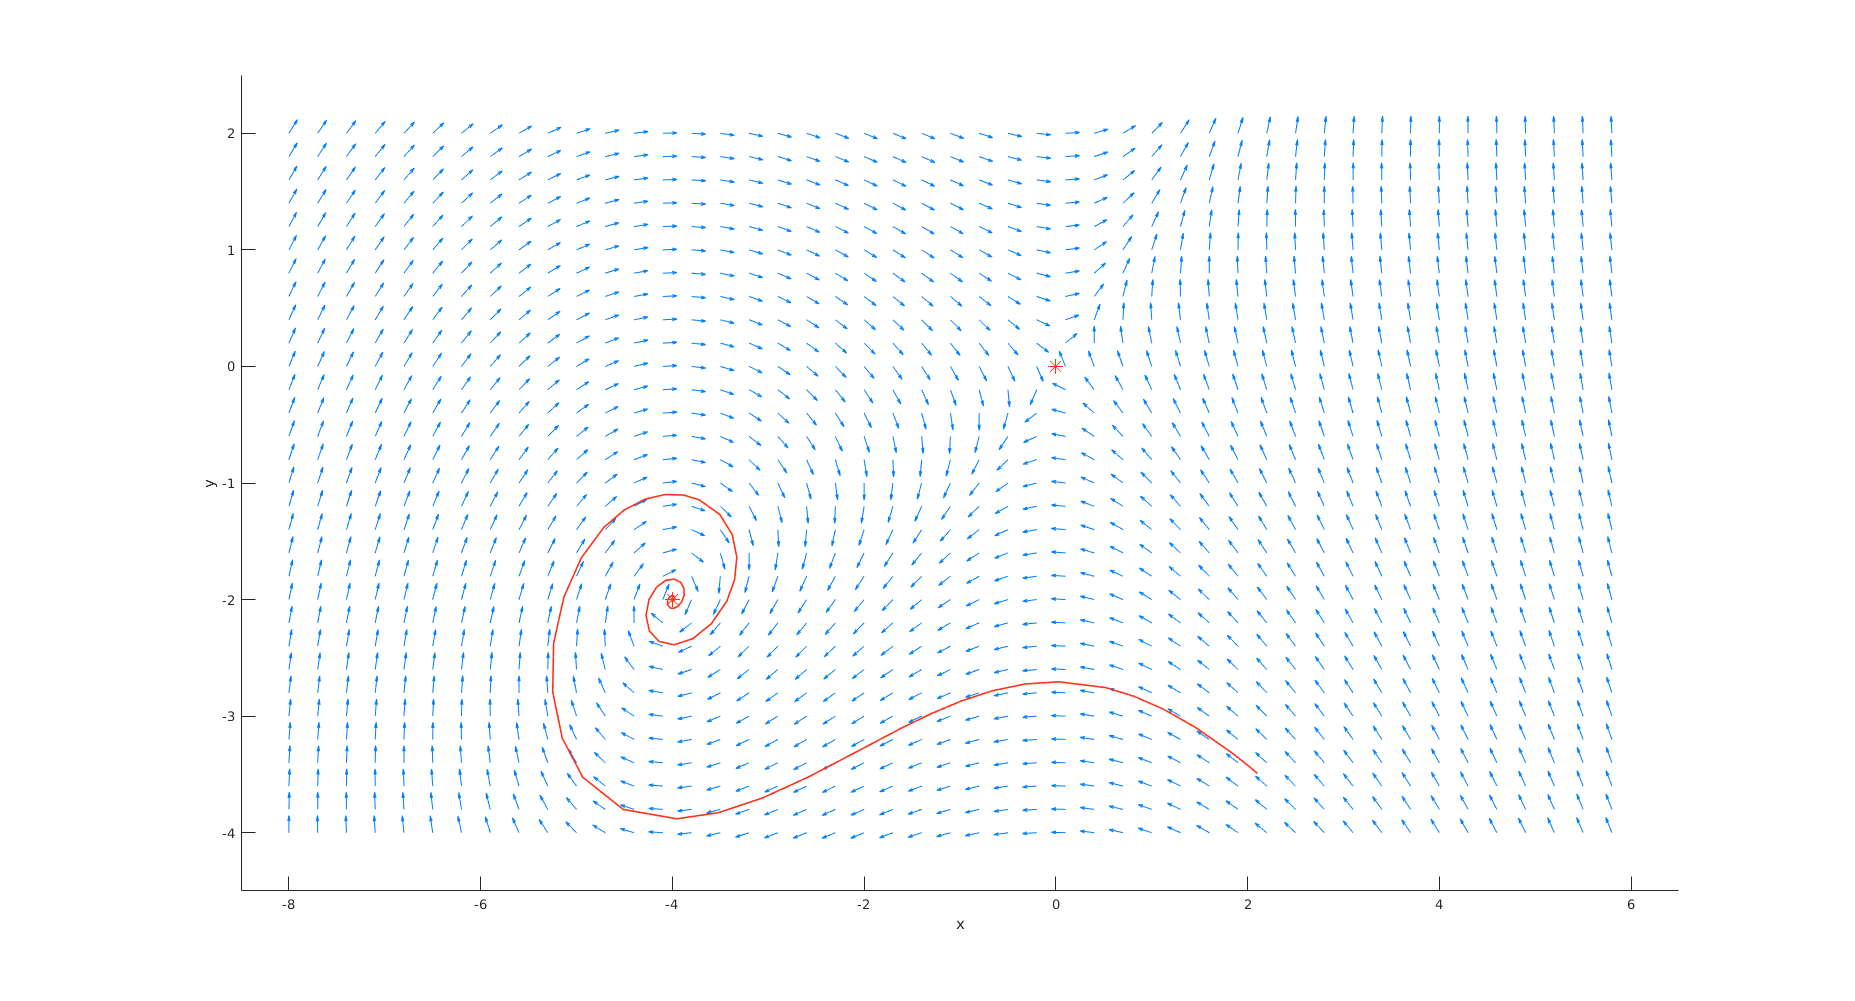
\includegraphics[width=\textwidth]{moveA.png}
    \caption{Фазова крива демонстираща асим. устойчивост на точката $(-4, \; -2)$}
\end{figure}

\begin{figure}[ht]
    \centering
    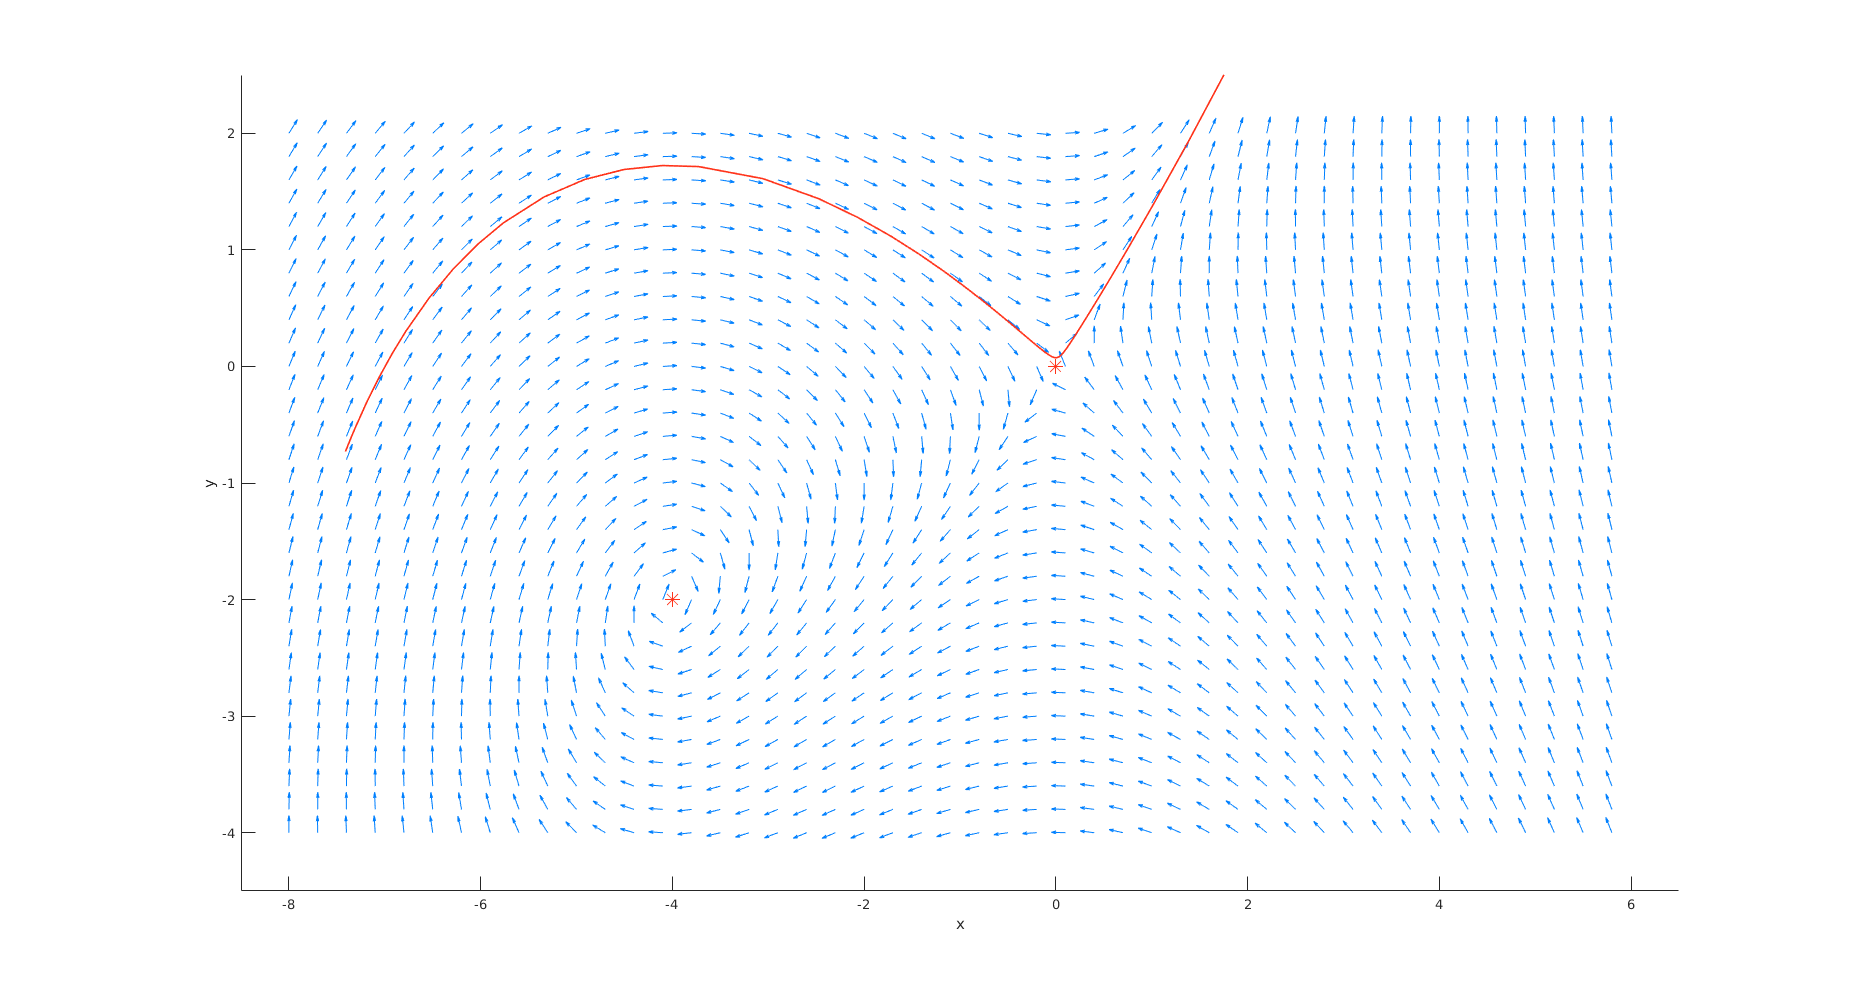
\includegraphics[width=\textwidth]{moveB.png}
    \caption{Една фазова крива демонстираща неустойчивостта на точката $(0, \; 0)$}
\end{figure}

\begin{figure}[ht]
    \centering
    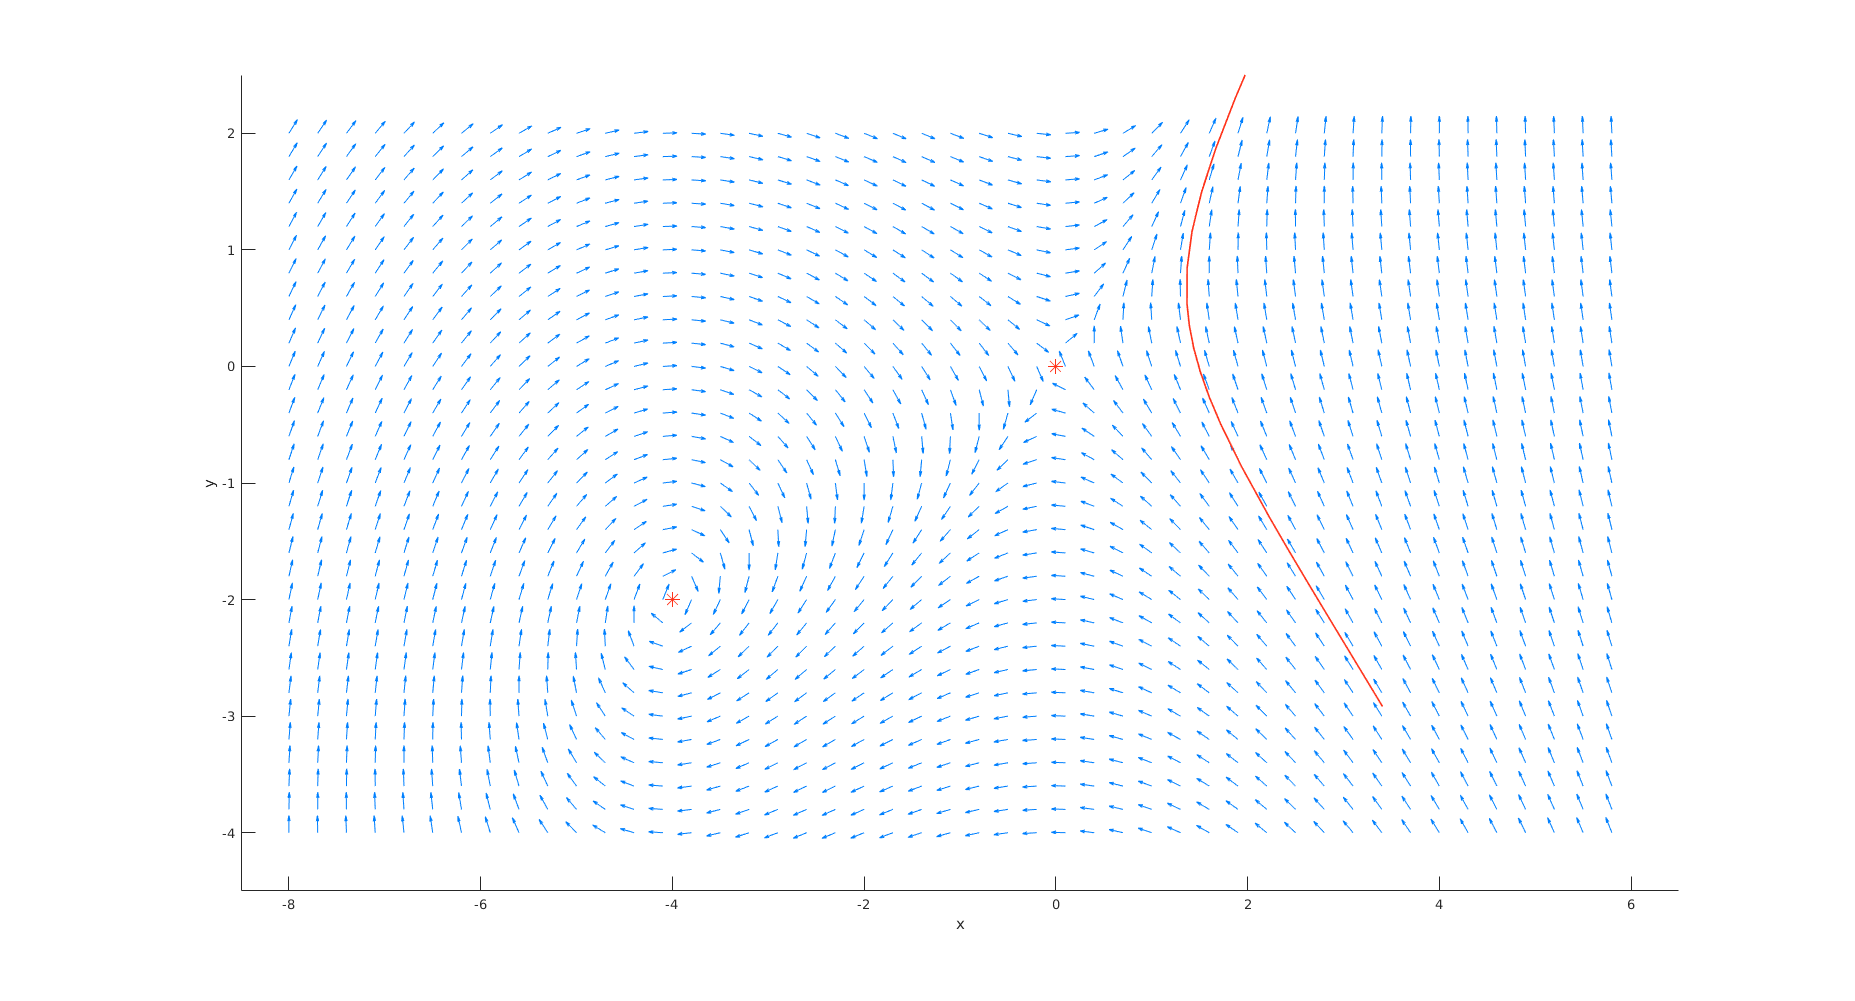
\includegraphics[width=\textwidth]{moveC.png}
    \caption{Друга фазова крива демонстираща неустойчивостта на точката $(0, \; 0)$}
\end{figure}

\subsection{Коментари към получените с Matlab резултати}
Фигури 3-11 показват кадри от анимацията на движението на точка
във фазовата равнина. Фигури 12-14 показват различни фазови криви.
Фигура 12 демонстрира асимптотическата устойчивост на точката $(-4, \; -2)$.
Фигури 13 и 14 демонстират неустойчивостта на точката $(0, \; 0)$.

\end{document}